\documentclass[11pt]{article}
\usepackage[margin=1in]{geometry}          
\usepackage{graphicx}
\usepackage{amsthm, amsmath, amssymb}
\usepackage{setspace}\onehalfspacing
\usepackage[loose,nice]{units}
\usepackage{array}
\usepackage[super]{nth}
\usepackage{graphicx}
\usepackage{float}
\usepackage{algpseudocode}
\usepackage[linesnumbered,ruled,vlined]{algorithm2e}
\usepackage{subcaption}
\usepackage{mathtools}
\usepackage[displaymath, mathlines]{lineno}
\usepackage{natbib}
% nicer math
\let\vec\mathbf
\usepackage[all]{nowidow}
\newenvironment{conditions}
  {\par\vspace{\abovedisplayskip}\noindent\begin{tabular}{>{$}l<{$} @{${}={}$} l}}
  {\end{tabular}\par\vspace{\belowdisplayskip}}
\newcommand{\R}{\mathbb{R}}  
\newenvironment{process}[1][htb]
  {\renewcommand{\algorithmcfname}{Process}% Update algorithm name
   \begin{algorithm}[#1]%
  }{\end{algorithm}}
\title{Role Model Choice Probability Regression}
\author{Saar Egozi and Yoav Ram}
\date{13/05/2020}

\begin{document}

\begin{titlepage}
\maketitle
\end{titlepage}

\section*{Role-Model Choice Process}
Consider a population of~$N$ role-models and copiers.
Copiers choose their role-models one by one.
We denote the number of copiers that chose role-model~$j$ after $i$~copiers have made their choice by $K_{i,j}$, such that $\sum_{j=1}^N{K_{i,j}} = i$. 
The stochastic process of role-model choice, 
\begin{equation} \label{eq:process}
\big\{\vec{K}_i\big\}_{i=1}^N, \quad \vec{K}_i=(K_{i,1}, \ldots, K_{i,N}),
\end{equation}
is described by the recurrence equation
\begin{equation} \label{eq:recurrence}
K_{i,j} = K_{i-1,j} + S_{i,j}, \quad i,j=1,2,\ldots,N
\end{equation}
where $S_{i,j}=1$ if the $i$-th copier chose role-model~$j$ and 0 otherwise, and the initial state is $K_{0,j}=0$.

The probability that the $i$-th copier chose role-model $j$
\begin{equation} 
G_{i,j}=P(S_{i,j}=1| S_{1,j},S_{2,j},...,S_{i-1,j})
\end{equation}
is called the \emph{prestige} of role-model~$j$ in the eyes of copier~$i$.
This prestige $G_{i,j}$ is determined as follows.
First, role-model~$j$ is characterised by its indicator value $A_j$.
Copier~$i$ estimates the indicator value of role-model~$j$, such that the estimated indicator value is
\begin{equation}
A_{i,j} = A_j + e_i,
\end{equation}
where $e_i$ is the estimation error of copier $i$. 
Then, a bias function is applied to the estimated indicator value,
\begin{equation}
\beta(A_{i,j}) = b \cdot \exp{\Big(-\frac{(A_{i,j} - \hat{A})^2}{2J}\Big)},
\end{equation}
where $\hat{A}$ is the optimal indicator value and $b,J$ are bias coefficients.
Finally, the prestige $G_{i,j}$ of role-model~$j$ in the eyes of copier~$i$ is determined by the estimated biased indicator value $\beta(A_{i,j})$ and the influence $K_{i-1,j}$, 
\begin{equation}\label{prestige_eq}
G_{i,j} = \frac{\alpha_j \cdot \beta(A_{i,j}) + (1-\alpha_j) \cdot K_{i-1,j}}{W_i},
\end{equation}
where the weight $\alpha_j$ is a characteristic of role-model~$j$ that determines the relative significance of the indicator and the influence in the prestige, and $W_i$ is a normalising factor to ensure $\sum_{j=1}^N{G_{i,j}}=1$,
\begin{equation}
W_i = \sum_{j=1}^N{\Big(\alpha_j \cdot \beta(A_{i,j}) + (1-\alpha_j) \cdot K_{i-1,j}\Big)}.
\end{equation}

In the following, we will analyse the stochastic process $\{\vec{K}_{i}\}_{I=1}^N$ to show the following results:
\begin{enumerate}
\item 
$K_{i,j}$ follows the general binomial distribution defined by \citep{GBD}.
Moreover, $\mathbb{E}[K_{N,j}] = N \cdot G_{1,j}$ if $e=e_l=e_m$ for all $l,m$.
 That is, the expected number of copiers of role-model~$j$ equals its prestige in the eyes of the first copier, multiplied by the total number of copiers. 
 In addition, we find that when $\alpha$ is homogenous, $\alpha_l=\alpha_m$ for all $l,m$, then $\mathbb{E}[K_{N,j}] = \beta(A'_j) \; / \; \overline{\beta(A') }$, where $A'_j$ is the estimated indicator value $A'_j=A_j+e$, and 
 $\overline{ \beta(A') }$ is the population mean estimated indicator value. 
 That is, the expected number of copiers of a role-model equals its relative biased indicator value, similar to the role of relative fitness in population-genetic models.
\item The role-model choice process (equation~\ref{eq:process}) is equivalent to a P\'{o}lya urn model if $e_l=e_m$ for all $l,m$. 
Therefore, $\vec{K}_i = (K_{i,1}, \ldots, K_{i,N})$ follows a Dirichlet-Multinomial distribution,
\begin{equation}
\vec{K}_i \sim \mathit{DM}\big(N, \vec{G}_1\big), 
\end{equation}
where $\vec{G}_1 = (G_{1,1}, \ldots, G_{1,N})$.
Note that here $G_{i,j}$ is only a function of the indicator values $A_j$ and the weights $\alpha_j$.
\end{enumerate}

\section*{General Binomial Distribution Approximation}
The general binomial distribution (GBD) is achieved by a series of Bernoulli experiments, with possible dependancy between experiments.
\paragraph{Proposition:} The number of copiers $K_{i,j}$ follows the GBD, $K_{i,j} \sim GBD(i,\alpha_i\cdot\beta(A'_j))$, when $e_l=e_m$ for all $l,m \in N$ and $A'_j=A_j + e$ 
\paragraph{Proof: } We'll denote $Q_j(k,i)=P(K_{i,j} = k | K_{i-1,j})$ as the probability that exactly $k$ out of $i$ copiers choose role-model $j$, using conditional probability and equation \ref{eq:recurrence}:
\begin{equation}\label{recursive}
Q_j(k,i) = P_j(S_{i,j}=1 | k-1,i-1) \cdot Q_j(k-1,i-1) + P_j(S_{i,j} =0 | k,i-1) \cdot Q_j(k,i-1)
\end{equation}
where $S_{i,j} =1 $ when the $i$-th copier chooses role-model $j$.

Equation \ref{recursive} is equivalent to equation 2.1 that \citet{GBD} define.
$Q_j(k,N)$ is the probability that $k$ out of $N$ copiers choose role-model $j$ at the end of the process, which by our previous notation is $k=K_{N,j}$.
By describing the process of equation \ref{eq:process} as \citep{GBD} did, we've completed the proof.

\paragraph{Corollary 1: } $\mathbb{E}[K_{N,j}] = N \cdot G_{1,j}$.\\
In \citep[equation 2.3]{GBD}, they show that the expected value of $k$ is: \\
$\mathbb{E}[k] = N \cdot Q_j(1,1)$ (using different notations).
$Q_j(1,1)$ is the initial probability to choose role-model $j$, before any choices are made.
$Q_j(1,1) = G_{1,j}$ by definition, therefore we can say that $\mathbb{E}[K_{N,j}]=N \cdot G_{1,j}$.\\

\paragraph{Corollary 2: } $\mathbb{E}[K_{Nj}] = \alpha_j \cdot \beta(A'_j) / \overline{\alpha \cdot \beta(A')}$.
\paragraph{Proof: } The initial prestige of role-model $j$ based on equation \ref{prestige_eq} is:
\begin{equation}\label{initial_prob}
G_{1,j} = \frac{\alpha_j\cdot\beta(A'_j)}{\sum\limits_{m=1}^{N}\alpha_m\cdot\beta(A'_m)}
\end{equation}
The denominator of equation \ref{initial_prob} can also be formulated as:
\begin{equation}\label{denominator}
 \sum\limits_{m=1}^{N}\alpha_m\beta(A'_m) = N \cdot \overline{\alpha \cdot \beta(A')}
\end{equation}
where $\overline{\alpha\beta(A')}$ is the mean value of $\alpha_m\cdot\beta(A'_m)$ for all $m$.
Using equation \ref{denominator} we get:
\begin{equation}
\mathbb{E}[K_{Nj}] = \alpha_j \cdot \beta(A'_j) \bigg/ \overline{\alpha \cdot \beta(A')}
\end{equation},
completing our proof.

The special case where $\alpha = \alpha_l=\alpha_m$ for all $l,m \in N$ is interesting, because we can evaluate the expected number of copiers using a linear equation:
\begin{equation}
\mathbb{E}[K_{Nj}]= N\cdot\frac{\alpha\cdot\beta(A'_j)}{\sum\limits_{m=1}^{N}\alpha\cdot\beta(A'_m)} =\beta(A'_j) \bigg/ \overline{\beta(A')}
\end{equation}
where the only variable is $A'_j$, because $\overline{\beta(A')}$ is the mean of the distribution we draw the indicator values from, modified by some constant parameters of $\beta$.
We can then denote $L = 1/\overline{\beta(A')}$ and write:

\begin{equation}\label{linearEq}
\mathbb{E}[K_{Nj}] = L\cdot \beta(A'_j)
\end{equation}

\begin{figure}
    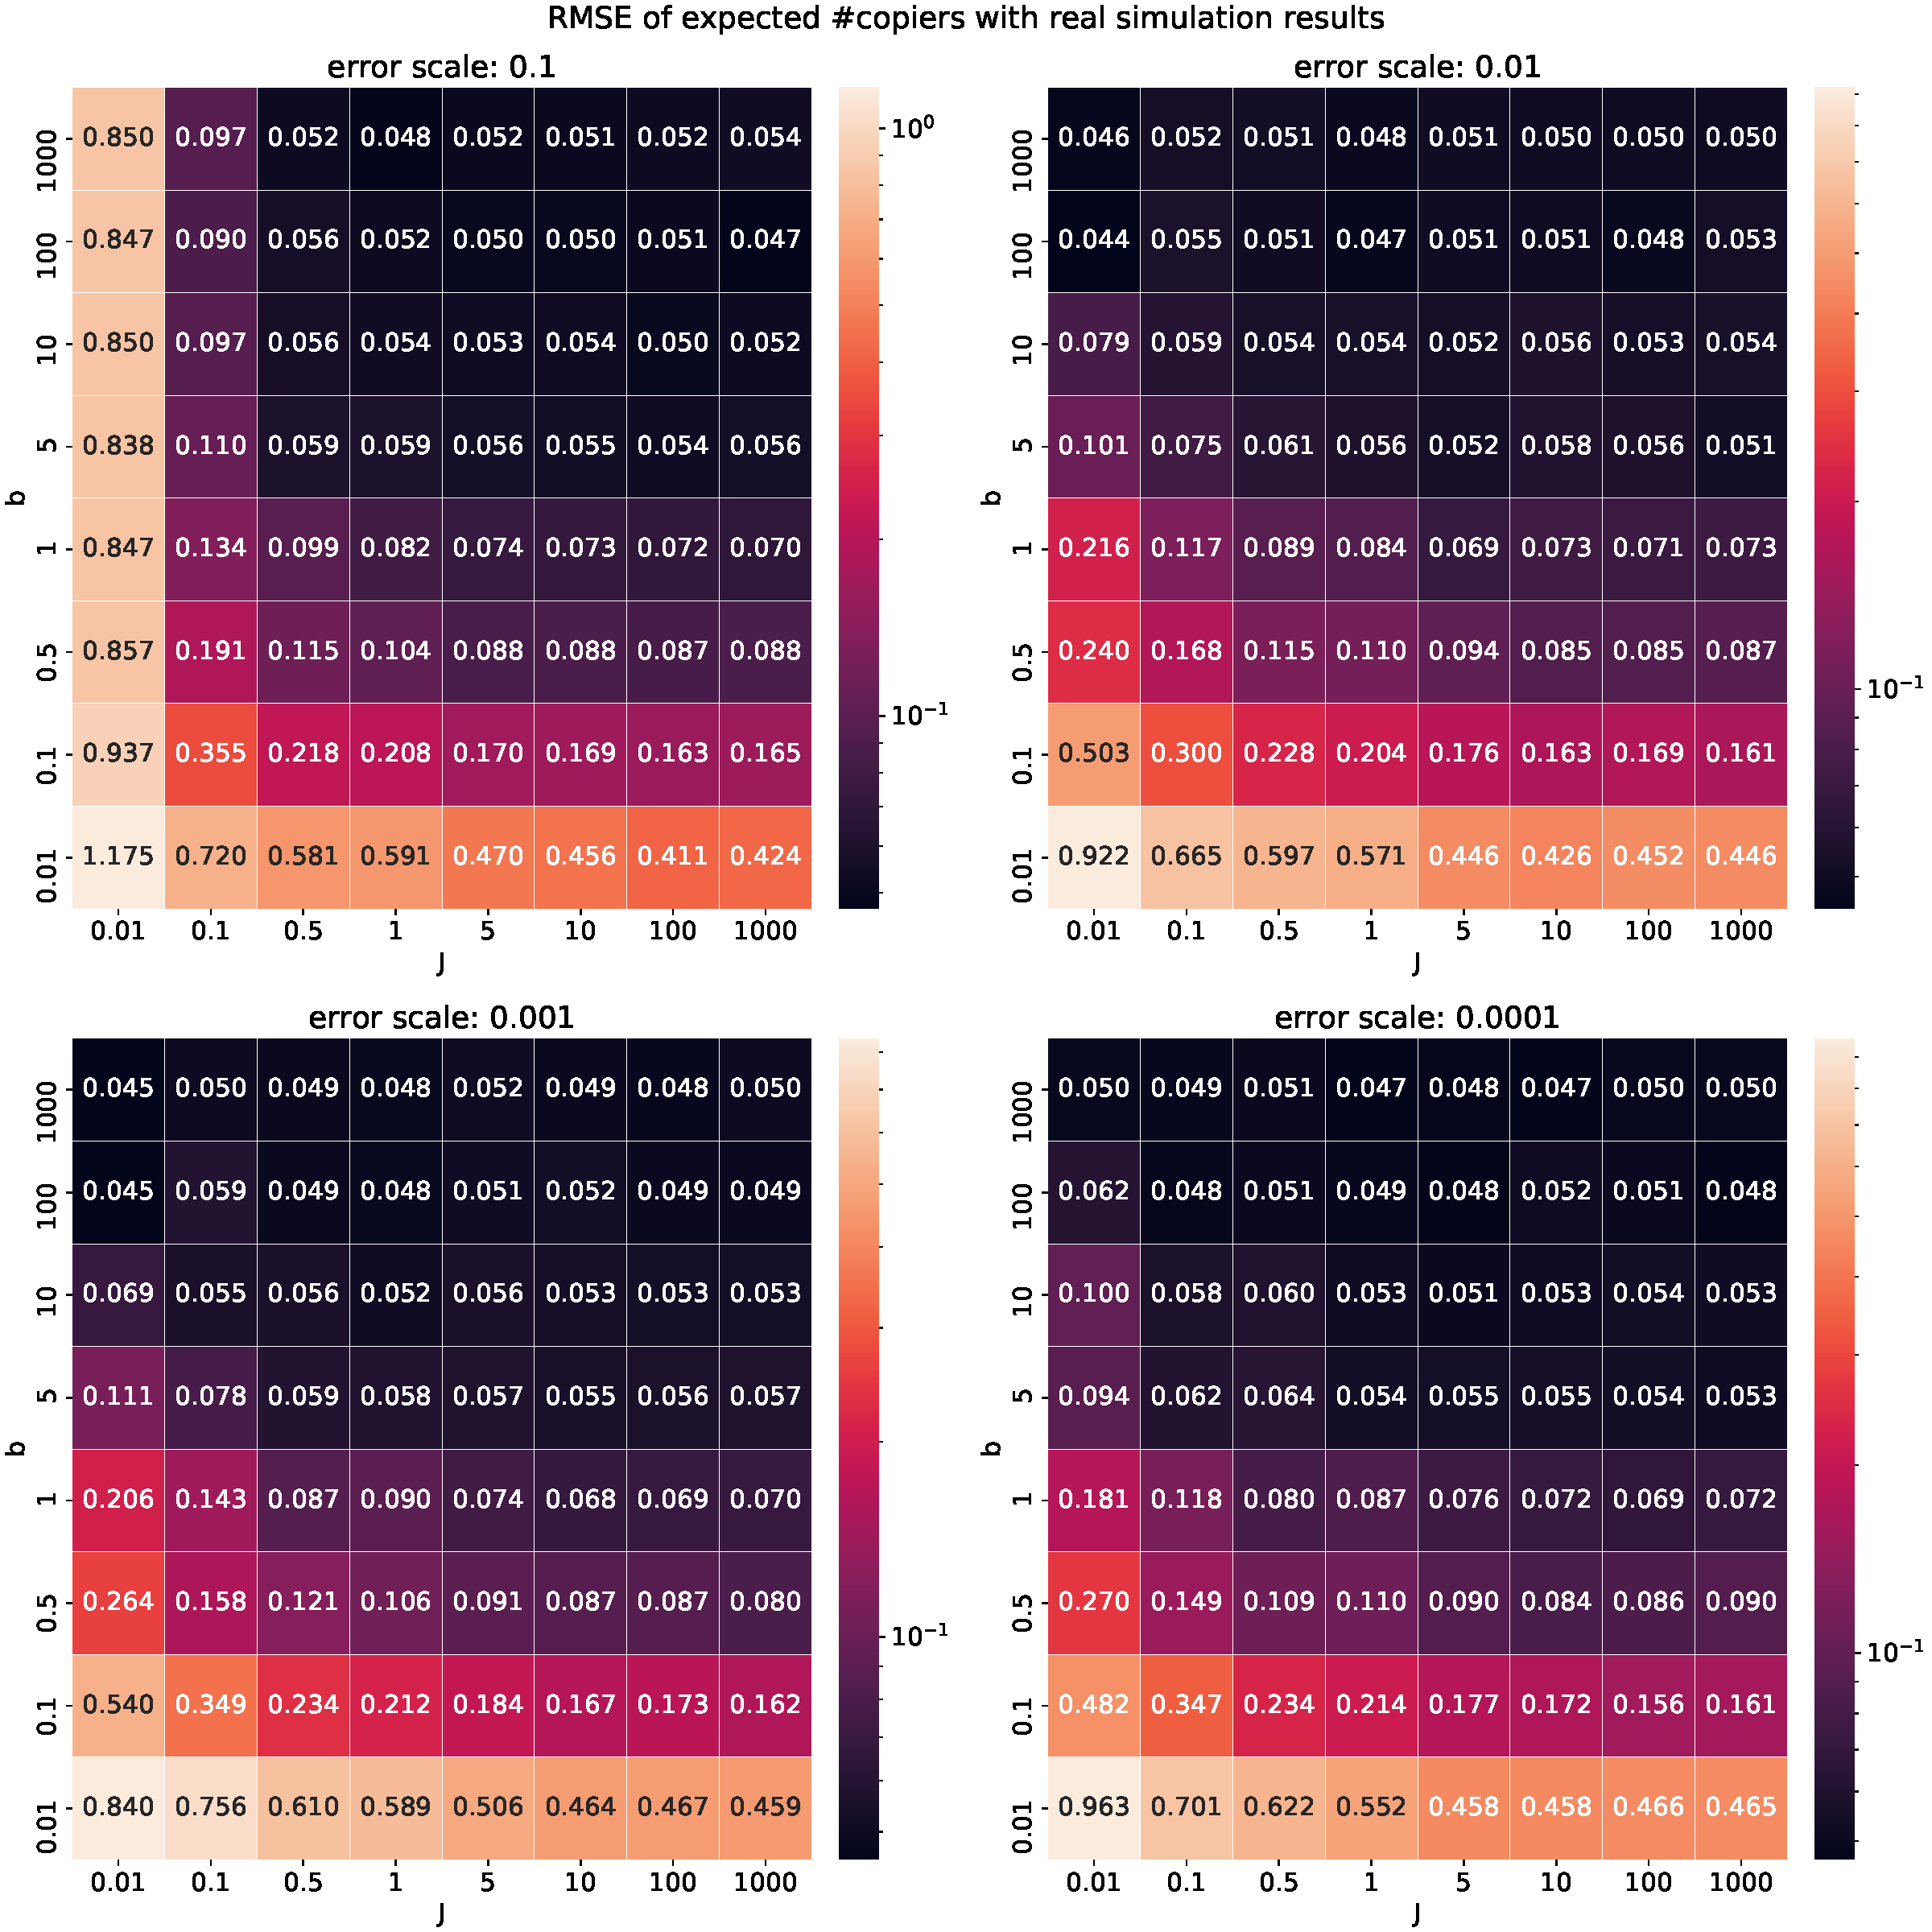
\includegraphics[width=\linewidth]{GBD_rmse_heatmap.pdf}
    \caption{RMSE graphs between the model results and the expected values based on equation \ref{linearEq}, for a population of $N=400$}
    \label{RMSE}
\end{figure}

\begin{figure}
    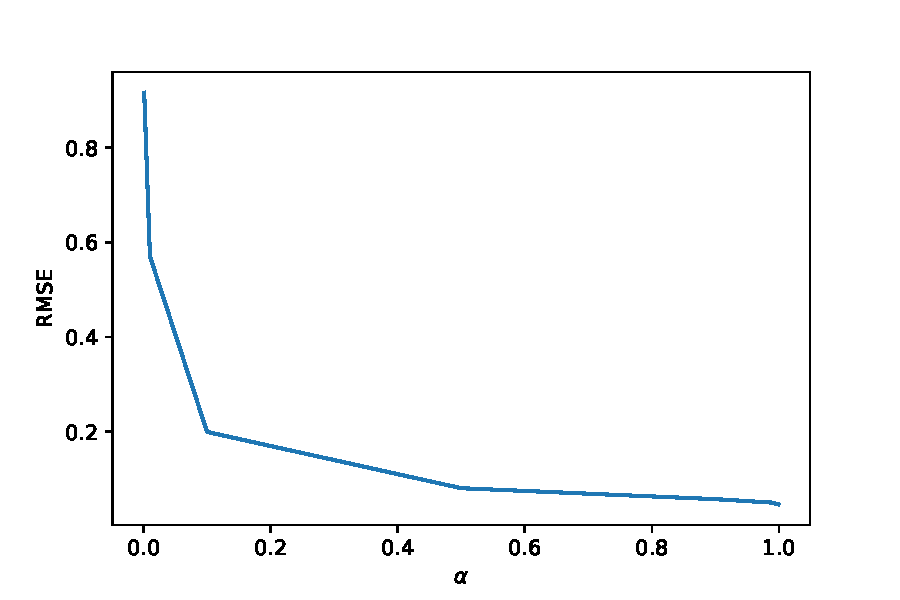
\includegraphics[width=\linewidth]{alpha_rmse.pdf}
    \caption{RMSE between the model results where $b=1,j=1,\eta=0.01$ and the expected values based on equation \ref{linearEq}, for a population of $N=400$}
    \label{RMSE:alpha}
\end{figure}

\paragraph{Numeric validation:} To validate our approximation for heterogenous estimation errors ($e_i \ne e_j$), we simulated process $\big\{\vec{K}_i\big\}_{i=1}^N$ 400 times over a population of 400 individuals.
We calculated the Root Mean Square Error (RMSE) between the average of the model's results and the expected values using equation \ref{linearEq}.
 We simulated the process for several values of: $b,J,\eta,\alpha$ ($e_i \sim N(0,\eta^2)$, $\alpha_l=\alpha_m$ for all $l,m$).
 In figure \ref{RMSE} we see that the RMSE is $\le 0.2$ in more than 70\% of the cases, and not more than 1.2 for any set of parameters.
 We can also see in figure \ref{RMSE:alpha} that for very small values of $\alpha$, the RMSE is still lower than 1. 
We consider these values acceptable because a deviation of 1 copier more or less for a large number of iterations is insignificant. 
We expect that the larger the population, and the larger the number of simulations, our approximation become more precise.
\clearpage

\section*{Dirichlet-Multinomial Distribution Approximation}
\paragraph{Reminder: \textit{Pólya urn model}}  is a stochastic process that is defined as such: 
The process consists of $N$ draws from an urn with an initial amount of coloured balls of $M$ colours. When a ball is drawn, it is then placed back in the urn together with an additional new ball of the same colour.\\
Let $\vec{U_i} = \{u_{i,1},u_{i,2},...,u_{i,M}\}$  where $u_{i,j}$ is the number of balls of the $j$-th colour in the urn after $i$ draws.
Let $S_{i,j}=1$ when drawing a $j$ coloured ball on the $i$-th draw, and $0$ otherwise. The probability that $S_{i,j}=1$ given $\vec{U_i}$ is:
\begin{equation}\label{polya}
\begin{split}
P(S_{i,j} = 1 | \vec{U_{i-1}}) & = \frac{u_{i-1,j}}{\sum\limits_{m=1}^{M} u_{i-1,m}} = \frac{o_j + w_{i-1,j}}{\sum\limits_{m=1}^{M} o_m + w_{i-1,m}}\\\\
 & = \frac{o_j + w_{i-1,j}}{i-1 + \sum\limits_{m=1}^{M} o_m}
\end{split}
\end{equation}
where $o_j$ is the initial number of balls of the colour $j$ in the urn, and $w_{i,j}$ is the number of new balls that were added to the urn after $i$ draws of the colour $j$.
Note that the initial number of balls in the urn process is discrete, but the process remains the same for a continuous amount.

\paragraph{Proposition:} process $\big\{\vec{K}_i\big\}_{i=1}^N$ is equivalent to a \textit{Pólya urn model} when $e=e_i=e_j$ and $\alpha=\alpha_j=\alpha_i$ for all $i,j \in N$.
\paragraph{Proof:} 
We denote $\alpha'$ as the odds ratio between the weights of the indicator and the influence ($\alpha'=\frac{\alpha}{1-\alpha}$). 
Using equation \ref{prestige_eq} we get:
\begin{equation}\label{copier_choose}
\begin{split}
G_{i,j} & = \frac{\alpha\cdot \beta(A'_j) + (1-\alpha) \cdot K_{i-1,j}}{W_i} \cdot \frac{1-\alpha}{1-\alpha} \\\\
&= \frac{\alpha'\beta(A'_j) + K_{i-1,j}}{\sum\limits_{m=1}^{N} \alpha'\beta(A'_m) + K_{i-1,m}}\\\\
& =\frac{\alpha'\beta(A'_j) + K_{i-1,j}}{i-1 + \sum\limits_{m=1}^{N} \alpha'\beta(A'_m)}
\end{split}
\end{equation}
Equations \ref{polya} and \ref{copier_choose} are equivalent when setting $M=N$, $o_j = \alpha'\beta(A'_j)$, $w_{i,j} = K_{i,j}$, completing the proof.

\paragraph{Corollary 1:}
In their paper, \citet[section 2]{dirichlet} prove that the proportion of different coloured balls in a \textit{Pólya urn model} will converge to the Dirichlet distribution as the number of draws approaches infinity, based on \textit{Martingale Convergence Theorem}. 
We can therefore sample from a Dirichlet-Multinomial distribution to approximate how many copiers each of the role-models will have:
$\vec{K_i} \sim DM(N,\vec{G_1})$.

\paragraph{Numeric validation:}
Fig. \ref{dirichlet_rmse} shows the root mean square errors between process $\big\{\vec{K}_i\big\}_{i=1}^N$ and a stochastic process that determines the number of copiers based on draws from the Dirichlet-Multinomial distribution.
We see that the RMSE are mainly around 0.07, and not larger than 1.2, same as before.

\paragraph{Corollary 2:} $\vec{K_i} \sim DM(N,\vec{G_1})$ for heterogenous indicator weight, $\alpha_l \ne \alpha_m$.
Our previous proof fails when $\alpha$ isn't homogenous, as can be seen in equation \ref{copier_choose}, because it is no longer equivalent to the \textit{Pólya urn} probability function (equation \ref{polya}).
We suggest that our approximation is still valid, as shown in Fig. \ref{hetero_alpha}

\begin{figure}
    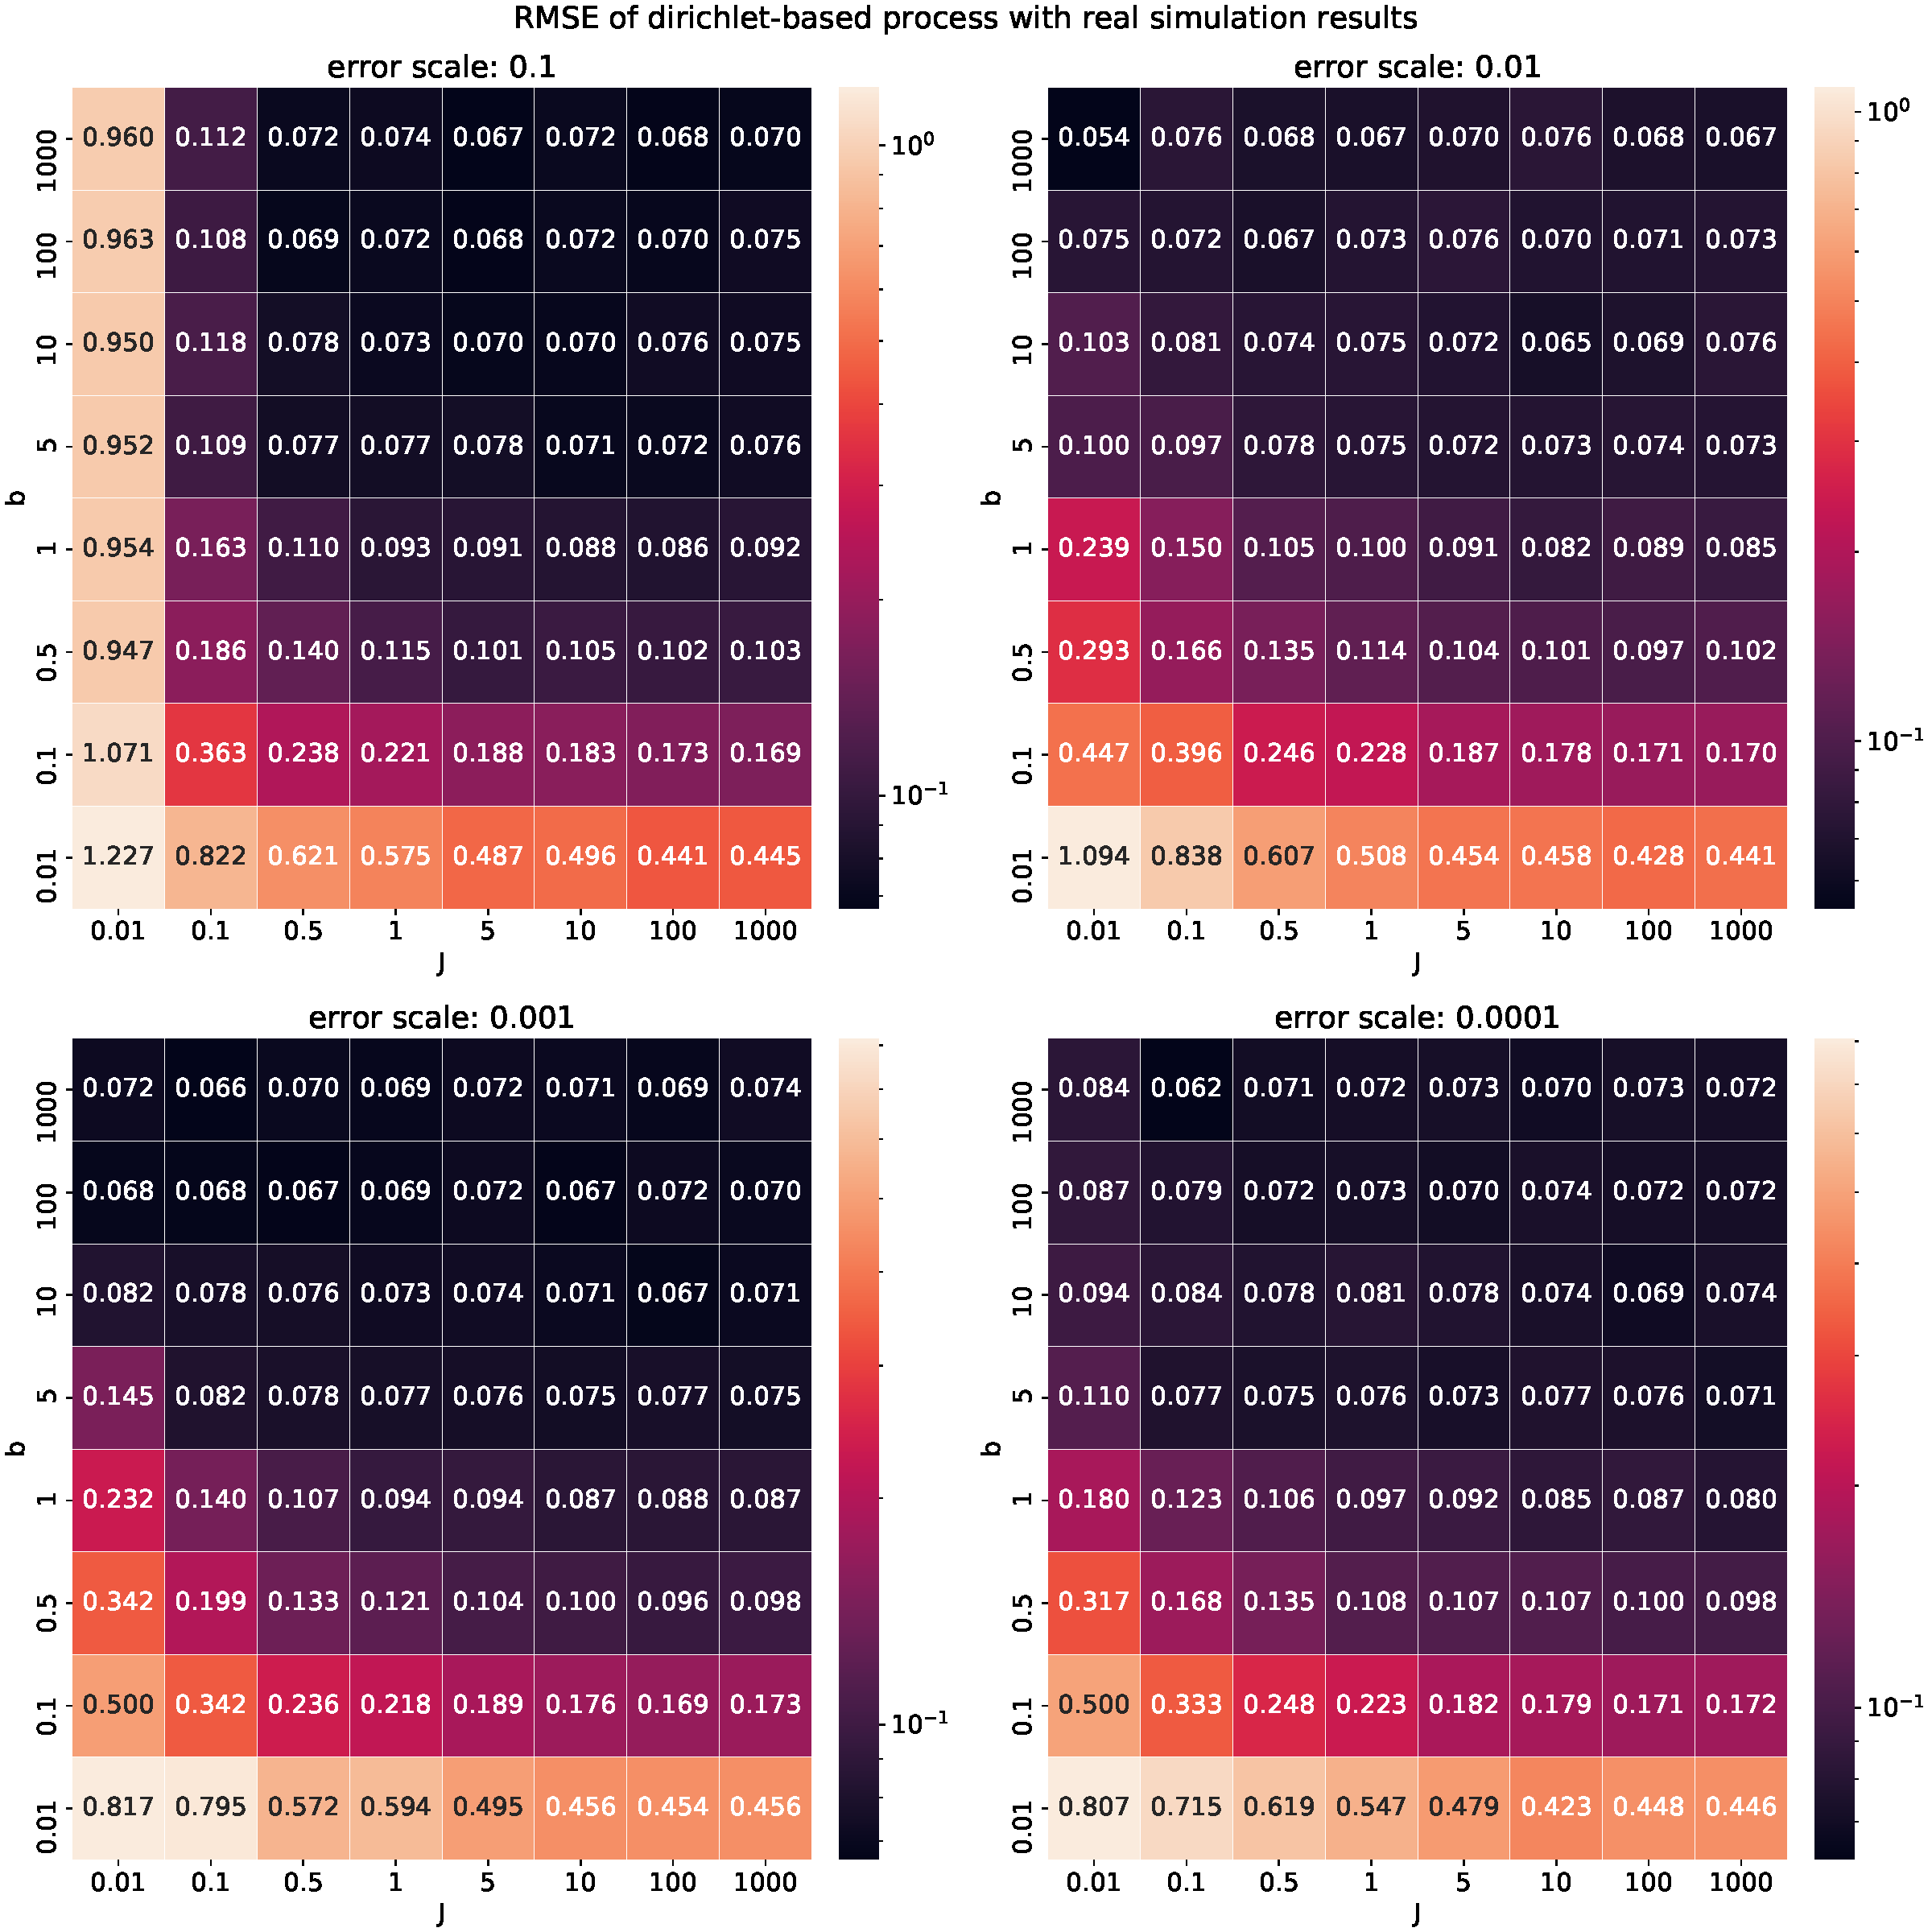
\includegraphics[width=\linewidth]{dirichlet_rmse_heatmap.pdf}
    \caption{RMSE graphs between the stochastic process by Algorithm 1 and a dirichlet-based process}
    \label{dirichlet_rmse}
\end{figure}



\clearpage
\bibliography{refs}
\bibliographystyle{apalike}
\end{document}